\section{Normality assessment using quantiles plots}\label{annexe:soil_desc_viz}

Figure~\ref{fig:soil-qq} presents the quantiles plots of the soil variables against a
theoretical normal distribution.

\textbf{COARSE} shows points following the reference line reasonably well, with
minor tail deviations, indicating slight non-normality.  
\textbf{SAND} displays strong deviation at high quantiles, confirming its
positively skewed, non-normal nature.  
\textbf{SILT} exhibits a pronounced S-shaped pattern, with clear departures in
both tails, indicating non-normality.  
\textbf{CLAY} aligns closely with the reference line, with only small deviations
at the extremes, and can be considered normally distributed.

\textbf{BULK} presents a clear right tail and upward deviation at high quantiles,
confirming non-normality.  
\textbf{REF\_BULK} closely follows the theoretical line across most quantiles,
indicating an approximately normal distribution.  
\textbf{ORG\_CARBON} shows mild curvature at the tails but remains largely
aligned, suggesting near-normal behavior.  
\textbf{PH\_WATER} shows strong deviations and non-linearity, indicating clear
departure from normality.

\textbf{TOTAL\_N} exhibits an almost linear pattern with slight deviations at
both tails, indicating slight normality.  
\textbf{CN\_RATIO} presents an S-shaped curve with upper-tail deviation,
confirming non-normality.  
\textbf{CEC\_SOIL} aligns well with the reference line, with only minor tail
effects, and can be considered normally distributed.  
\textbf{CEC\_CLAY} shows slight upward deviation in the upper tail but otherwise
follows the line, indicating slight normality.

\textbf{CEC\_EFF}, \textbf{TEB}, \textbf{BSAT}, \textbf{ALUM\_SAT},
\textbf{ESP}, \textbf{GYPSUM} and \textbf{ELEC\_COND} all exhibit strong curvature
and substantial deviations from the reference line, confirming pronounced
right-skewed and non-normal distributions.  
\textbf{TCARBON\_EQ} shows relatively good alignment with mild upper-tail
deviation, indicating slight normality.

These results confirm that most soil variables do not follow a Gaussian
distribution and will require appropriate transformations or robust scaling
prior to statistical modelling.

\begin{figure}[H]
    \centering
    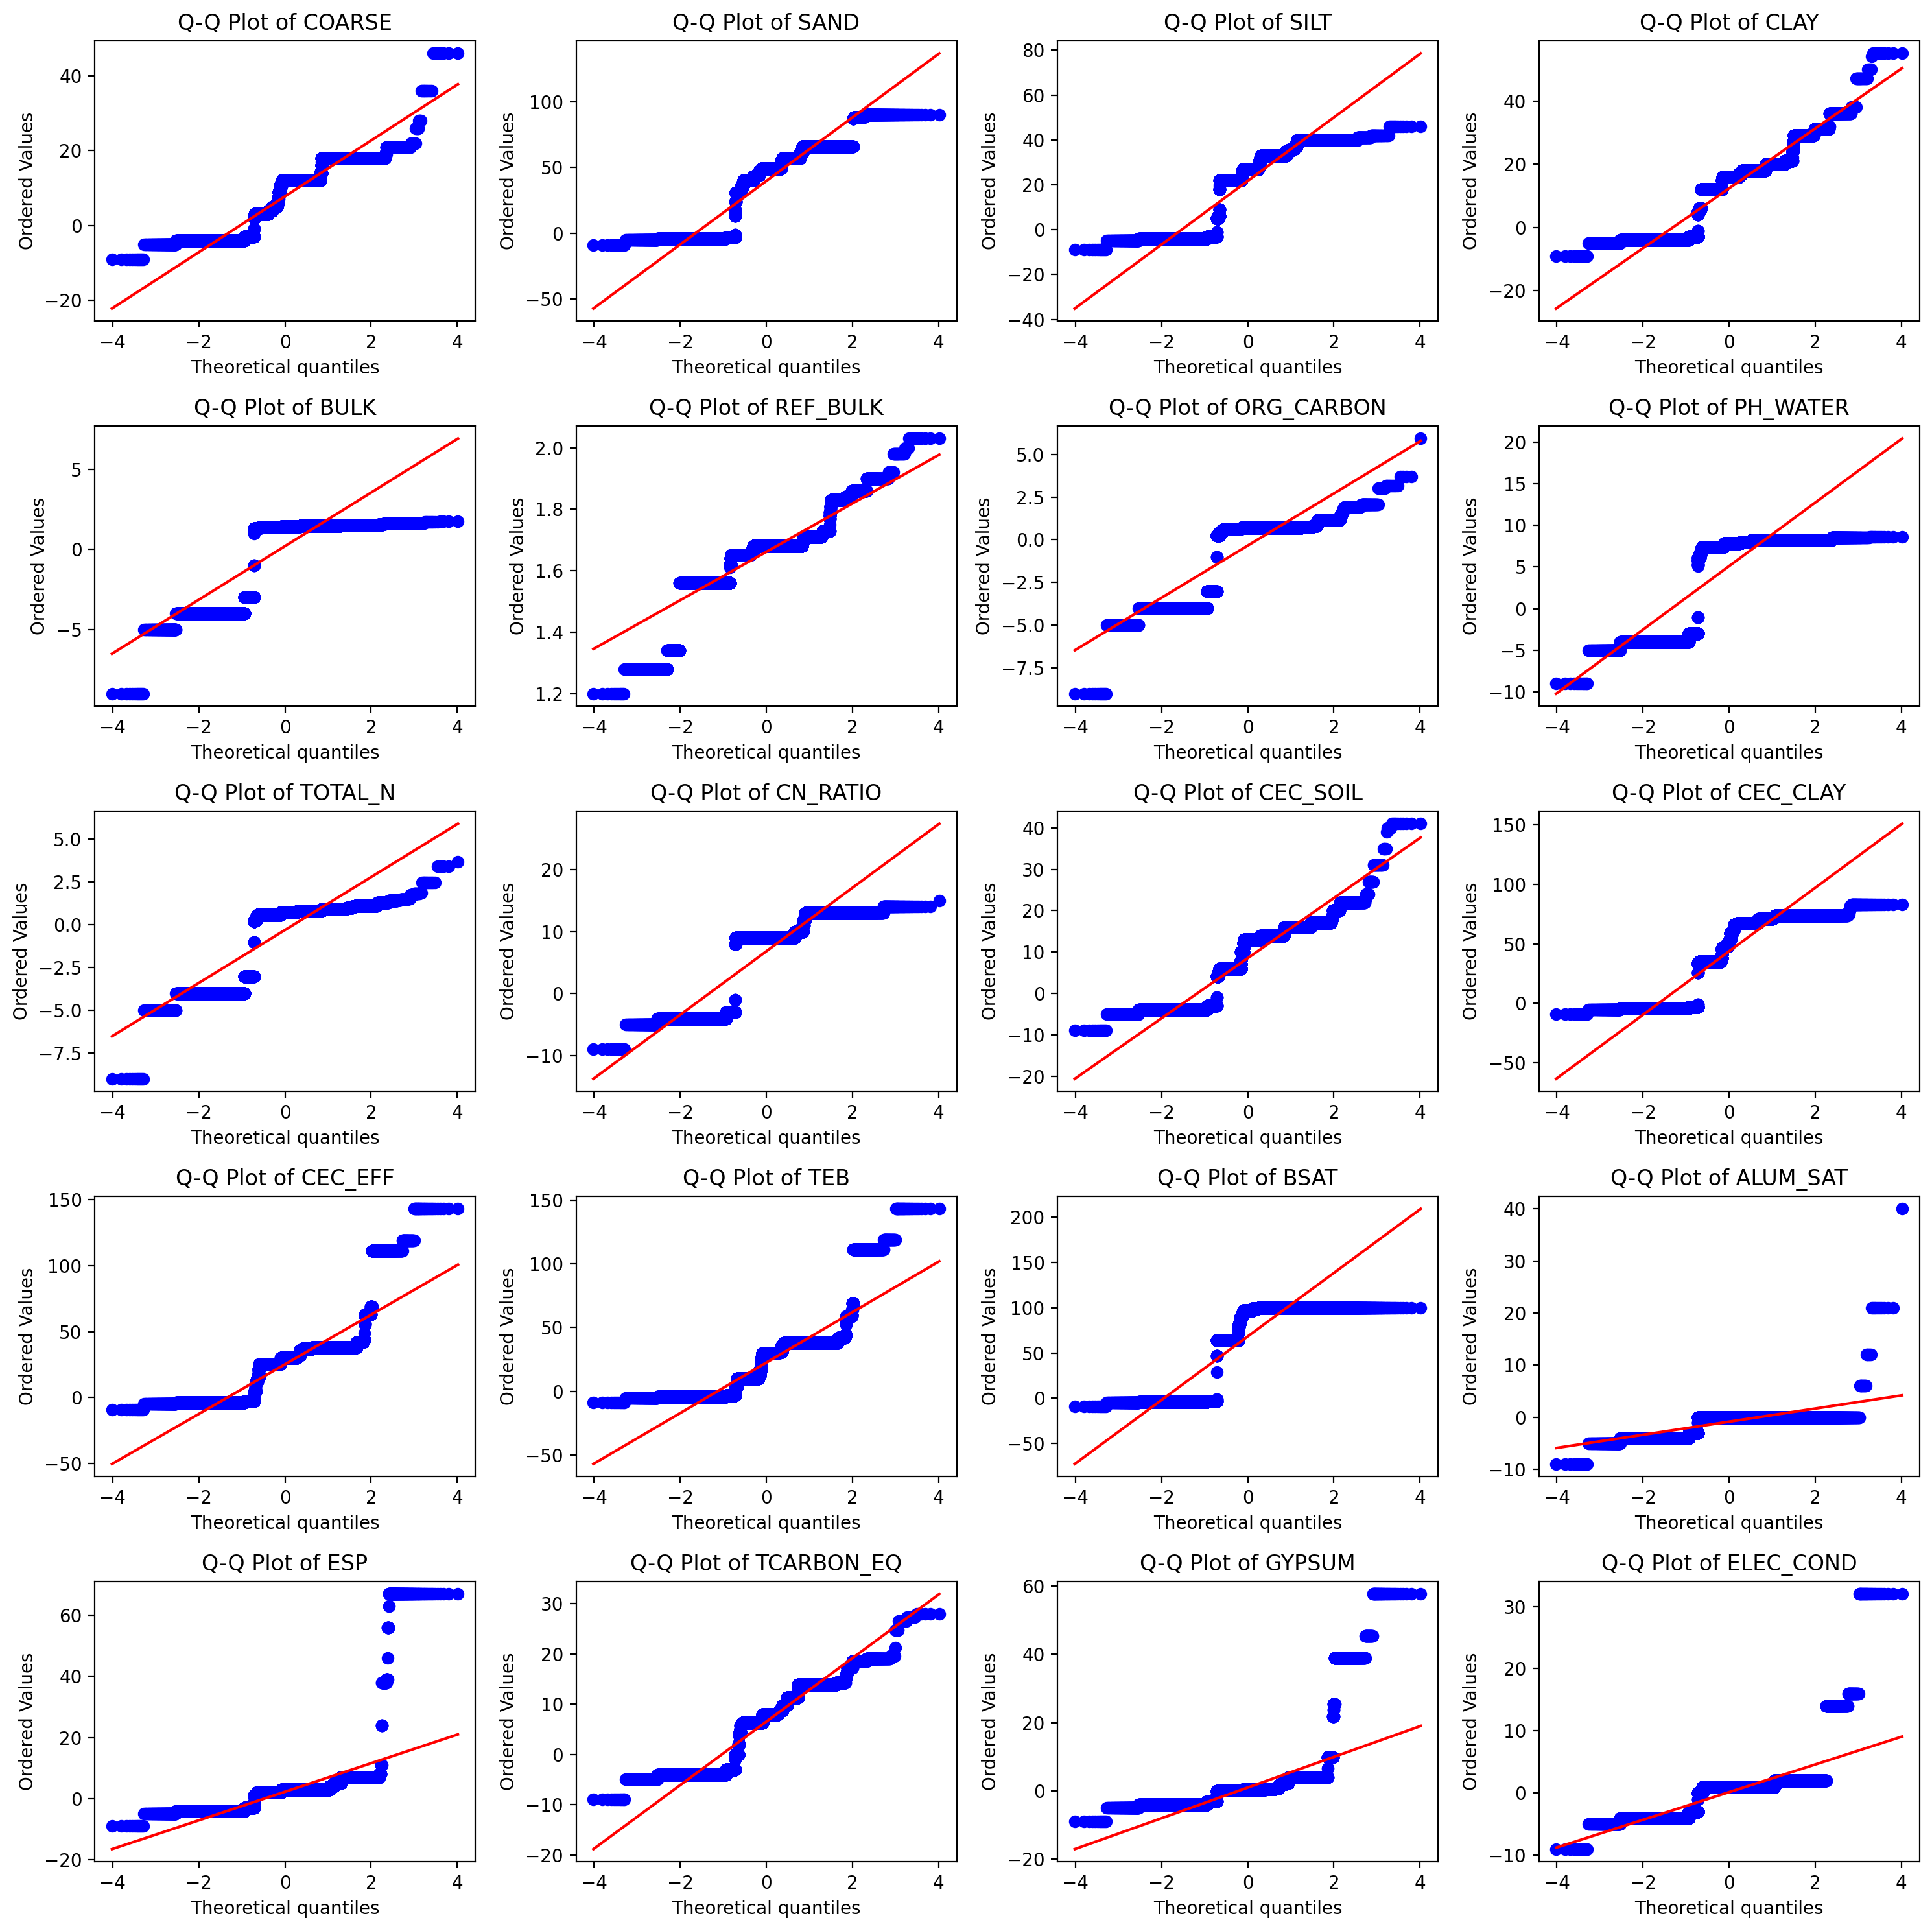
\includegraphics[width=0.65\textwidth]{images/Soil/soil_qq_numeric}
    \caption{Quantiles plots of soil numeric variables against the normal
    distribution.}\label{fig:soil-qq}
\end{figure}
